\section{Appendix C: Additional figures}
\label{app:figures}

\begin{figure}[H]
\centering
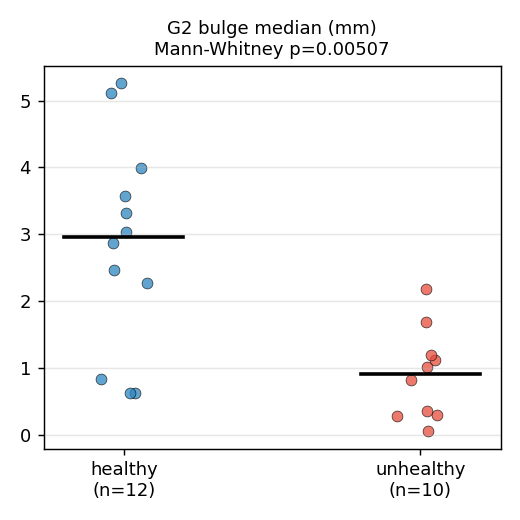
\includegraphics[width=0.45\textwidth]{figures/bulge-med.png}
\caption{Group 2 posterior disc bulge (median per case), healthy vs.\ unhealthy. The metric reads
\emph{backwards} --- healthy shows a higher bulge than the symptomatic cohort --- one of the two
sign-level disc-metric bugs the validation harness detected (Section~\ref{sec:results},
Section~\ref{sec:g2}). Retained as evidence rather than hidden.}
\label{fig:bulge}
\end{figure}

\noindent The remaining per-measure strip plots appear in Figure~\ref{fig:strips}
(Section~\ref{sec:results}). All figures are regenerated from
\texttt{run\_validation\_master.py} (matplotlib), and the architecture diagram (Figure~\ref{fig:pipeline})
is drawn in TikZ so it requires no external image file.
